\documentclass{beamer}
\usetheme{Madrid}
\usecolortheme{beaver}
\usepackage{tikz}
\usepackage{xcolor}
\usepackage{booktabs}
\usetikzlibrary{positioning}

\title{Friedrich Nietzsche's Ethics}
\subtitle{Beyond Good and Evil}
\author{Brendan Shea, PhD}
\date{\today}

\begin{document}

\begin{frame}
\titlepage
\end{frame}

\begin{frame}{Introduction: Friedrich Nietzsche and His Ethical Thought}
\begin{itemize}
\item Friedrich Nietzsche (1844-1900) was one of the most radical and influential philosophers of the 19th century.
\item His ethical philosophy challenges traditional morality at its foundations, questioning its assumptions and origins.
\item Nietzsche rejects universal moral codes in favor of a focus on human excellence and individual flourishing.
\item His ideas remain controversial, widely misunderstood, and often challenging for beginning readers.
\end{itemize}

\begin{alertblock}{Key Question}
What if conventional morality is not beneficial for all human beings, but actually prevents some from achieving their full potential?
\end{alertblock}
\end{frame}

\begin{frame}{Who Was Nietzsche? A Brief Biography}
\begin{itemize}
\item Born in Prussia in 1844, Nietzsche was the son of a Lutheran pastor who died when Friedrich was only five years old.
\item He became the youngest professor of classical philology at the University of Basel at age 24, before health issues forced him to retire.
\item From 1879 until 1889, Nietzsche lived as an independent philosopher, writing his most important works.
\item In January 1889, he suffered a mental collapse and spent his final silent years in the care of his mother and sister until his death in 1900.
\end{itemize}

\begin{center}
\scriptsize
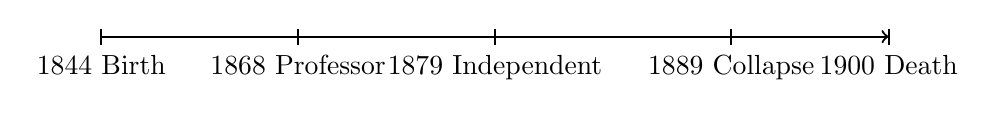
\begin{tikzpicture}
\draw[thick, ->] (0,0) -- (10,0);
\foreach \x/\label in {0/1844 Birth, 2.5/1868 Professor, 5/1879 Independent, 8/1889 Collapse, 10/1900 Death}
    \draw[thick] (\x,0.1) -- (\x,-0.1) node[below] {\label};
\end{tikzpicture}
\end{center}
\end{frame}

\begin{frame}{Nietzsche's Writing Style: Provocative and Aphoristic}
\begin{itemize}
\item Nietzsche deliberately avoided writing systematic philosophical treatises, preferring a more literary approach.
\item He wrote in an \textbf{aphoristic style} - short, dense paragraphs expressing complete thoughts that reward careful reading.
\item His tone is often provocative, using hyperbole, metaphor, and shocking statements to challenge readers' assumptions.
\item Nietzsche wants to shake readers awake rather than merely present arguments for intellectual consideration.
\end{itemize}

\begin{exampleblock}{Example from \textit{Beyond Good and Evil}}
``Gradually it has become clear to me what every great philosophy has been: namely, the personal confession of its author and a kind of involuntary and unconscious memoir; also that the moral (or immoral) intentions in every philosophy constituted the real germ of life from which the whole plant has grown.''
\end{exampleblock}
\end{frame}


\begin{frame}{The Historical Context: Post-Enlightenment Europe}
    \begin{itemize}
    \item Nietzsche wrote during a time of significant cultural and intellectual transition in Europe, as traditional religious authority declined.
    \item The rise of science, industrialization, and democratic movements were reshaping society and challenging old values.
    \item The phrase \textbf{"God is dead"} captures Nietzsche's recognition that European culture was losing its religious foundations.
    \item He saw both dangers and opportunities in this transition, warning of potential nihilism but also the chance for new values.
    \end{itemize}
    
    \begin{block}{Historical Influences}
    \begin{itemize}
    \item Ancient Greek culture (especially pre-Socratic philosophers)
    \item German Romanticism and idealism
    \item Arthur Schopenhauer's pessimism
    \item Darwin's evolutionary theory
    \end{itemize}
    \end{block}
    \end{frame}
    
    \begin{frame}{Key Works in Nietzsche's Ethics}
    \begin{itemize}
    \item \textit{Human, All Too Human} (1878): Nietzsche's first work to directly criticize morality and religion.
    \item \textit{The Gay Science} (1882): Introduces the "death of God" and eternal recurrence concepts.
    \item \textit{Thus Spoke Zarathustra} (1883-1885): Fictional narrative presenting Nietzsche's most famous ideas.
    \item \textit{On the Genealogy of Morality} (1887): His most sustained critique of conventional morality's historical development.
    \end{itemize}
    
    \begin{table}
        \scriptsize
    \begin{tabular}{ll}
    \toprule
    \textbf{Early Period} & Classical philology, influence of Wagner and Schopenhauer \\
    \midrule
    \textbf{Middle Period} & Break with earlier influences, focus on psychology and critique \\
    \midrule
    \textbf{Late Period} & Most influential ethical works, revaluation of values \\
    \bottomrule
    \end{tabular}
    \end{table}
    \end{frame}
    
    \begin{frame}{What Makes Nietzsche's Ethics Different?}
    \begin{itemize}
    \item Unlike Kant or utilitarians, Nietzsche does not provide a systematic theory of right action or moral rules.
    \item He offers a \textbf{critique of morality itself}, questioning its origin, value, and effects on human flourishing.
    \item Nietzsche employs a \textbf{genealogical method}, examining how moral concepts developed historically rather than assuming their eternal truth.
    \item His approach is descriptive and evaluative rather than prescriptive, focusing on psychological and cultural analysis.
    \end{itemize}
    
    \begin{center}
    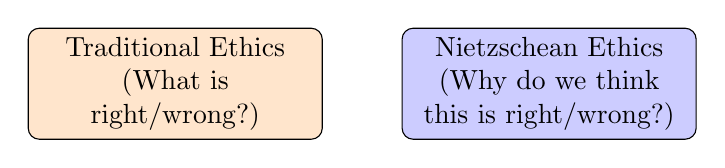
\begin{tikzpicture}
    \node[draw, rectangle, rounded corners, fill=orange!20, text width=3.5cm, align=center] (a) {Traditional Ethics\\(What is right/wrong?)};
    \node[draw, rectangle, rounded corners, fill=blue!20, text width=3.5cm, align=center, right=1cm of a] (b) {Nietzschean Ethics\\(Why do we think this is right/wrong?)};
    \path[->] (a) -- (b);
    \end{tikzpicture}
    \end{center}
    \end{frame}
    
    \begin{frame}{Nietzsche's Big Question: What's Wrong with Morality?}
    \begin{itemize}
    \item Nietzsche asks: What if conventional morality is harmful to the flourishing of exceptional individuals?
    \item He challenges us to reexamine our moral assumptions rather than just accepting them as given.
    \item Morality might be useful for maintaining social order but could constrain human excellence and creativity.
    \item His critique is not about rejecting all values but questioning whether our current values serve human flourishing.
    \end{itemize}
    
    \begin{alertblock}{Central Claim}
    "What if a symptom of regression lurked in the 'good'... So that morality itself were to blame if the highest power and splendor possible to the type man was never in fact attained?" (GM Preface:6)
    \end{alertblock}
    \end{frame}

    \begin{frame}{Understanding "Morality in the Pejorative Sense" (MPS)}
        \begin{itemize}
        \item Nietzsche doesn't criticize all forms of ethics or values, but targets what he calls \textbf{"morality in the pejorative sense"} (MPS).
        \item MPS refers specifically to moral systems that claim universal authority and prioritize values like equality, altruism, and pity.
        \item Examples of MPS include Christian morality, Kantian ethics, and utilitarianism, which all share certain problematic features.
        \item Nietzsche believes these moralities emerged from particular historical and psychological conditions, not universal truths.
        \end{itemize}
        
        \begin{block}{Characteristics of MPS}
        \begin{itemize}
        \item Claims universal authority ("one morality for all")
        \item Promotes selflessness, altruism, and equality
        \item Devalues self-interest, ambition, and competition
        \item Presents itself as objective and beyond questioning
        \end{itemize}
        \end{block}
        \end{frame}
        
        \begin{frame}{Descriptive vs. Normative Components of Morality}
        \begin{itemize}
        \item Nietzsche identifies two components in moral systems that he critiques separately.
        \item The \textbf{descriptive component} consists of claims about human nature, agency, and psychology that morality presupposes.
        \item The \textbf{normative component} consists of the specific values and judgments that a moral system promotes.
        \item Both components are problematic for Nietzsche, but for different reasons.
        \end{itemize}
        
        \begin{table}
        \centering
        \begin{tabular}{|c|c|}
        \hline
        \textbf{Component} & \textbf{Description} \\
        \hline
        Descriptive Component & False claims about human nature \\
        \hline
        Normative Component & Harmful values for higher types \\
        \hline
        \end{tabular}
        \caption{Components of Morality in the Pejorative Sense}
        \end{table}   
    \end{frame}
        
        \begin{frame}{Critique \#1: The Problem with Free Will}
        \begin{itemize}
        \item Morality assumes that humans have \textbf{free will} - the ability to choose actions independently of causal determination.
        \item Nietzsche rejects this, arguing that our choices are determined by unconscious psychological and physiological factors.
        \item The idea that we are consciously "choosing" our actions is an illusion; our consciousness is largely epiphenomenal.
        \item Without free will, moral responsibility (praise and blame) loses its foundation.
        \end{itemize}
        
        \begin{exampleblock}{Nietzsche's View}
        "The 'inner world' is full of phantoms... The will no longer moves anything, hence does not explain anything either - it merely accompanies events; it can also be absent." (Twilight of the Idols)
        \end{exampleblock}
        \end{frame}
        
        \begin{frame}{The "Doctrine of Types": How We're Shaped by Nature}
        \begin{itemize}
        \item Nietzsche proposes what scholars call the \textbf{"Doctrine of Types"} - the view that each person has a fixed psycho-physical constitution.
        \item This constitution consists of unconscious drives, affects, and physiological factors that largely determine who we are.
        \item Our conscious thoughts, values, and beliefs arise from these deeper type-facts rather than from rational deliberation.
        \item Different human types flourish under different conditions, making universal moral prescriptions problematic.
        \end{itemize}
        
        \begin{alertblock}{Key Insight}
        "Our moral judgments and evaluations... are only images and fantasies based on a physiological process unknown to us." (Daybreak 119)
        \end{alertblock}
        \end{frame}

\end{document}